\section*{What has been done this week}
%\textit{\textbf{Hint:}Try to write this section so it can be used directly in your thesis. Also use drawings and figures.}


\newpage
\section{Metric performance}


\subsection{Variance of Laplacian}
% generate plots with outlier from new dataset and update in report
This metric has been implemented for both jpg and png filetypes.

\textbf{Outlier}
An outlier in the sharp images have been discovered. As can be seen in the image below, a few images are classified as much sharper than the rest of the images with a score of around 6 compared to the rest of the scores around 1.
\begin{figure}[H]
	\centering
    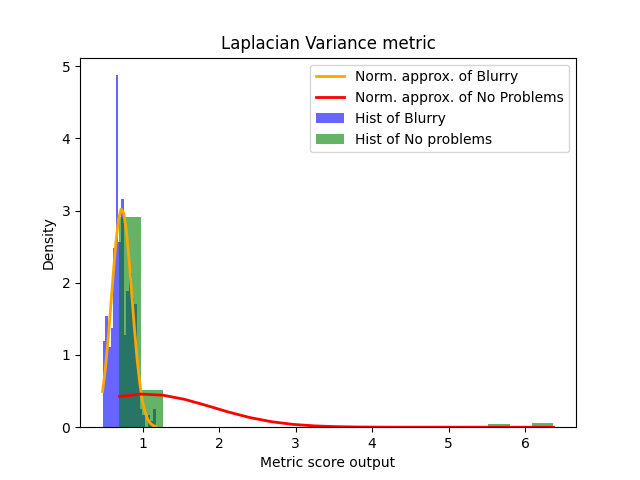
\includegraphics[width=.8\textwidth]{Figures/lv/output_dens_lv_jpg_old.png}
    \caption{\textcolor{red}{update diagram* }A density plot on the training data of filetype jpg. The true blurry images are visualized in the blue histogram and the orange pdf-curve, and the sharp images are vizualised by the green histogram and the red pdf-curve. No gaussian blurred images have been included.}
    \label{fig:LV_dens_jpg_old}
\end{figure}

Displaying the image after applying the laplacian filter in the algorithm produces the output displayed in figure \ref{fig:LV_very_sharp}.

\begin{figure}[H]
    \centering
    \begin{subfigure}[t]{0.48\textwidth}
	    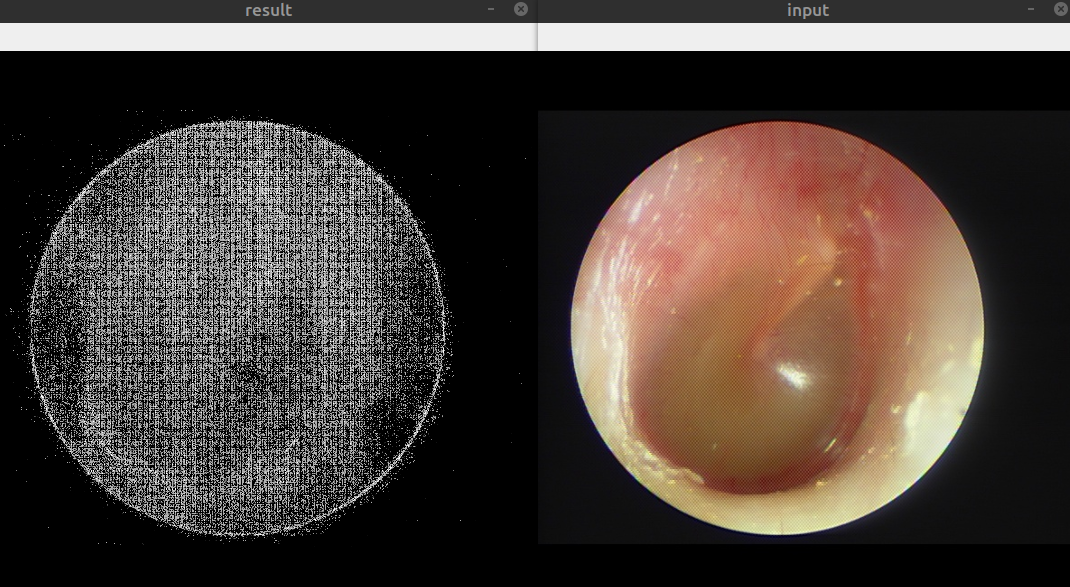
\includegraphics[width=\textwidth]{Figures/lv/lv_33_png.png}
	    \caption{The right image is the input image of type png. The left image is the result of applying a laplacian filter on it.}
    \end{subfigure}\hspace{1em}
    \begin{subfigure}[t]{0.48\textwidth}
    		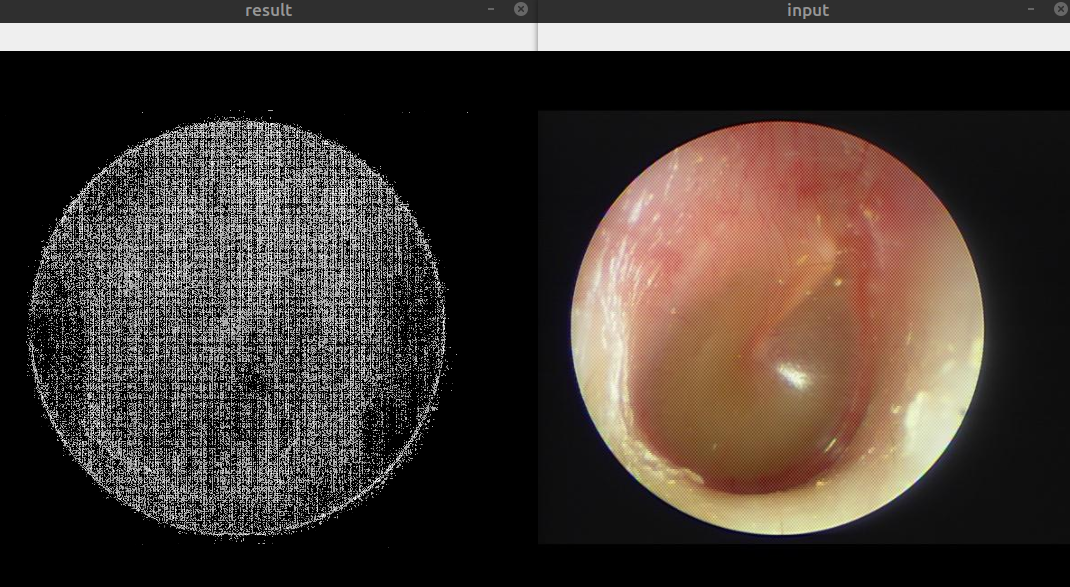
\includegraphics[width=\textwidth]{Figures/lv/lv_33_jpg.png}
    		\caption{The right image is the input image of type jpg. The left image is the result of applying a laplacian filter on it.}
    \end{subfigure}\hspace{1em}
%    \label{fig:LV_dens_jpg_old}

    \begin{subfigure}[t]{0.48\textwidth}
	    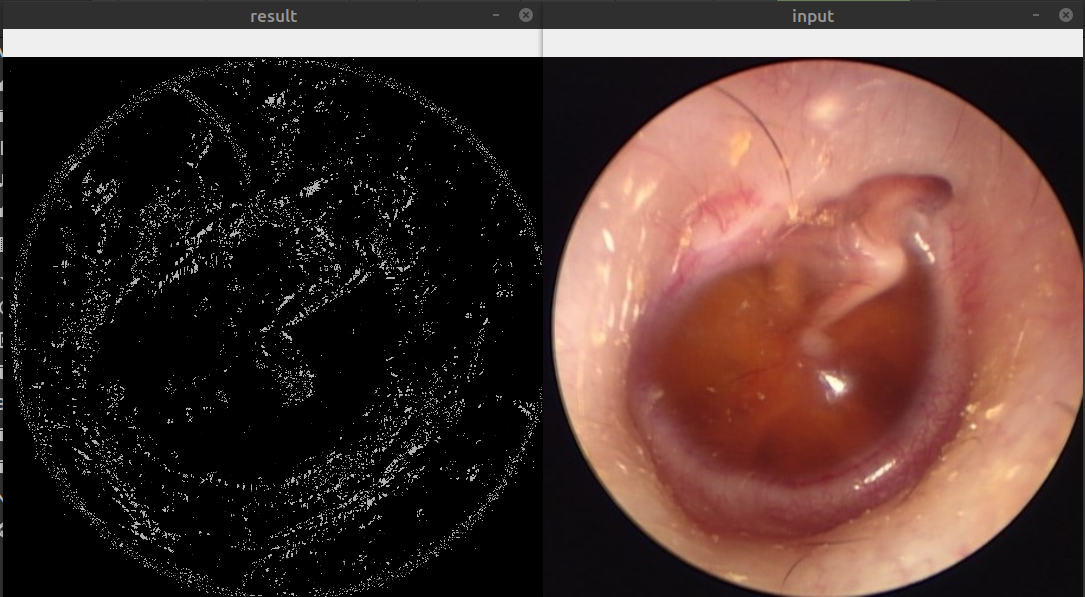
\includegraphics[width=\textwidth]{Figures/lv/out_29_png.png}
	    \caption{The right image is the input image of type png. The left image is the result of applying a laplacian filter on it.}
    \end{subfigure}\hspace{1em}
    \begin{subfigure}[t]{0.48\textwidth}
    		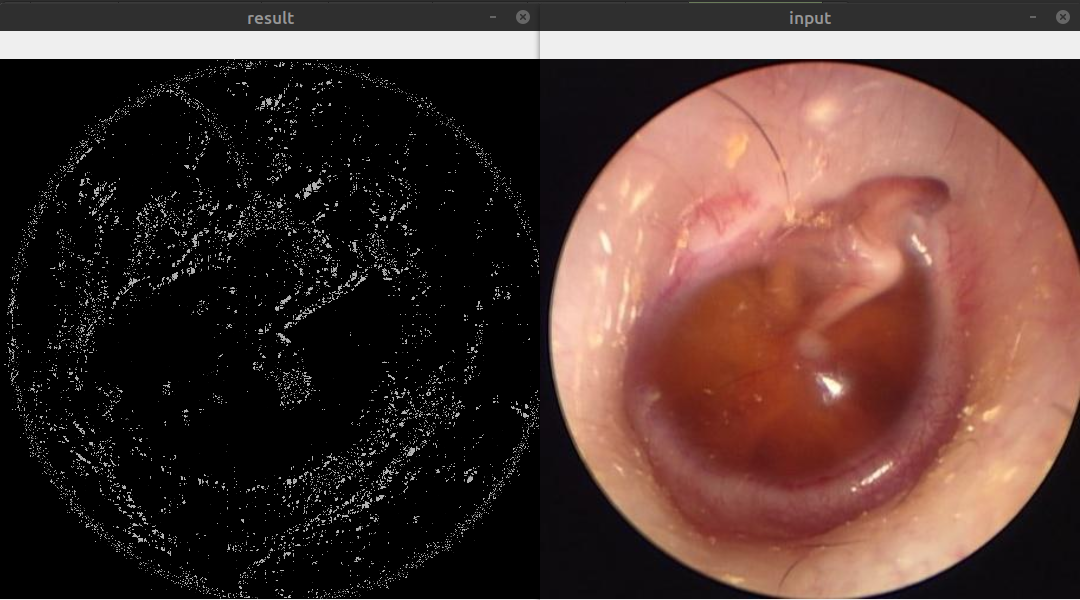
\includegraphics[width=\textwidth]{Figures/lv/out_29_jpg.png}
    		\caption{The right image is the input image of type jpg. The left image is the result of applying a laplacian filter on it.}
    \end{subfigure}\hspace{1em}
    \caption{The above images displays the laplacian output of two different true sharp images of filetype png and jpg. The lower images represent a normal output of the laplacian filter, while the upper images produces outliers.}
    \label{fig:LV_very_sharp}
\end{figure}

Looking closely at the original image (both jpg and png), one can see a filter-like pattern, which produces the very white output.

\begin{figure}[H]
    \centering
    \begin{subfigure}[t]{0.48\textwidth}
	    \centering
	    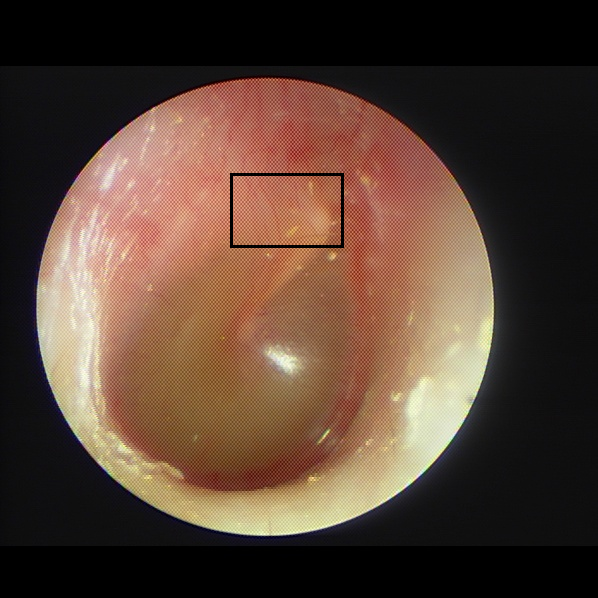
\includegraphics[height=.66\textwidth]{Figures/lv/33.png}
	    \caption{}
    \end{subfigure}\hspace{1em}
    \begin{subfigure}[t]{0.48\textwidth}
	    \centering
	    
\includegraphics[height=.66\textwidth]{Figures/lv/33_zoom.png}
	    \caption{}
    \end{subfigure}\hspace{1em}
\end{figure}

This image and the synthetic sharp data produced from it will be disregarded from the following analysis.


\textbf{JPG}
\begin{figure}[H]
    \centering
    \begin{subfigure}[t]{0.48\textwidth}
        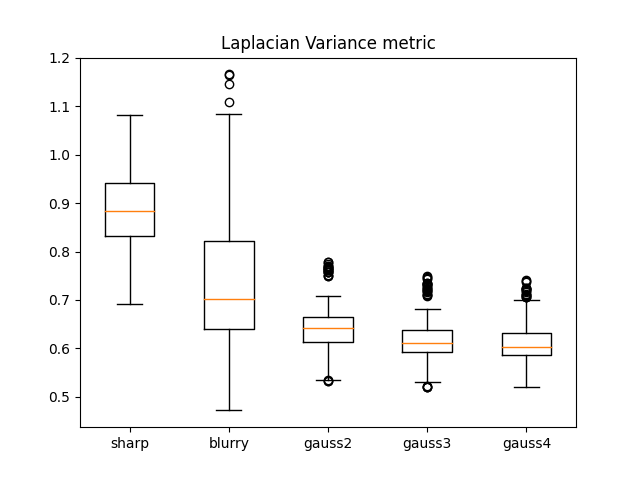
\includegraphics[width=\textwidth]{Figures/lv/output_boxplot_lv_jpg.png}
        \caption{}
        \label{fig:LV_roc}
    \end{subfigure}\hspace{1em}
    \begin{subfigure}[t]{0.48\textwidth}
	    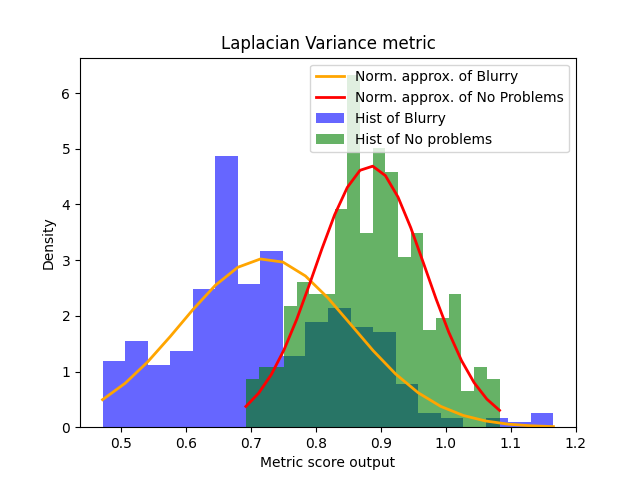
\includegraphics[width=\textwidth]{Figures/lv/output_dens_lv_jpg.png}
	    \caption{}
	    \label{fig:LV_dens_jpg}
    \end{subfigure}\hspace{1em}

    \begin{subfigure}[t]{0.48\textwidth}
        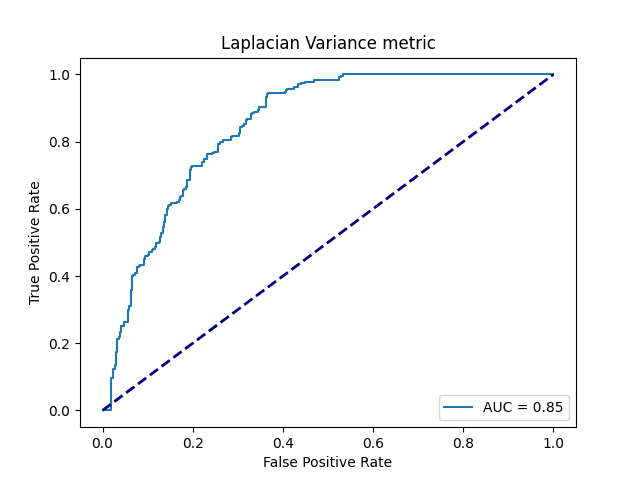
\includegraphics[width=\textwidth]{Figures/lv/output_roc_lv_jpg.png}
        \caption{}
        \label{fig:LV_roc}
    \end{subfigure}\hspace{1em}
    \begin{subfigure}[t]{0.48\textwidth}
        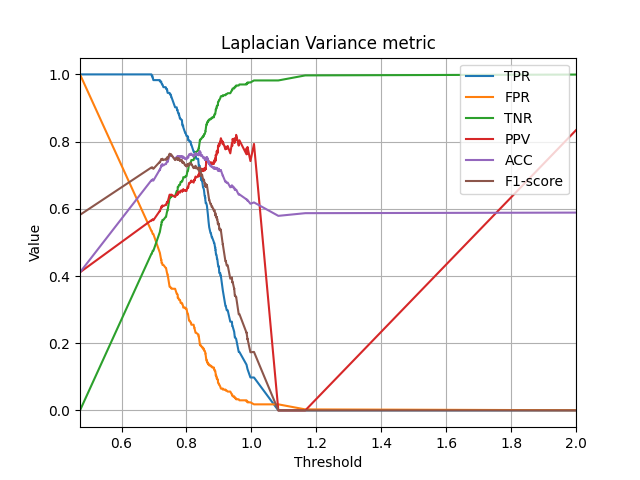
\includegraphics[width=\textwidth]{Figures/lv/threshold_test_scores_lv_jpg.png}
        \caption{}
        \label{fig:LV_thresh}
    \end{subfigure}\hspace{1em}
    \caption{}
    \label{fig:LV_final}
\end{figure}


\textbf{PNG}
\begin{figure}[H]
    \centering
    \begin{subfigure}[t]{0.48\textwidth}
        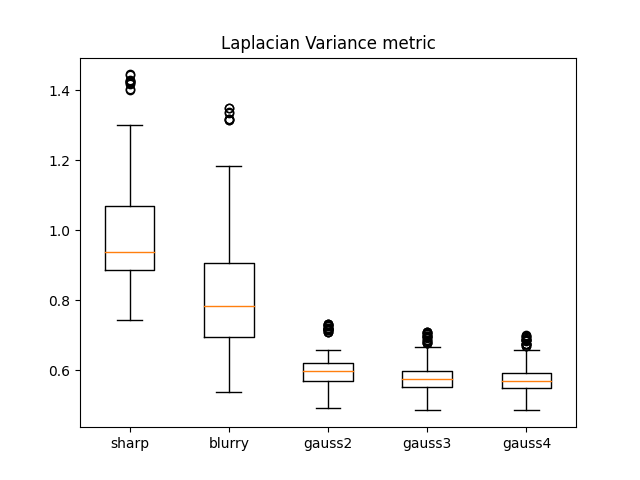
\includegraphics[width=\textwidth]{Figures/lv/output_boxplot_lv_png.png}
        \caption{}
        \label{fig:LV_roc}
    \end{subfigure}\hspace{1em}
    \begin{subfigure}[t]{0.48\textwidth}
	    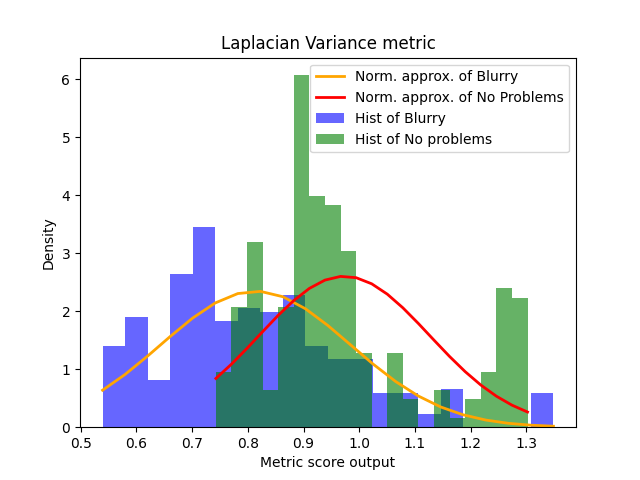
\includegraphics[width=\textwidth]{Figures/lv/output_dens_lv_png.png}
	    \caption{}
	    \label{fig:LV_dens_png}
    \end{subfigure}\hspace{1em}

    \begin{subfigure}[t]{0.48\textwidth}
        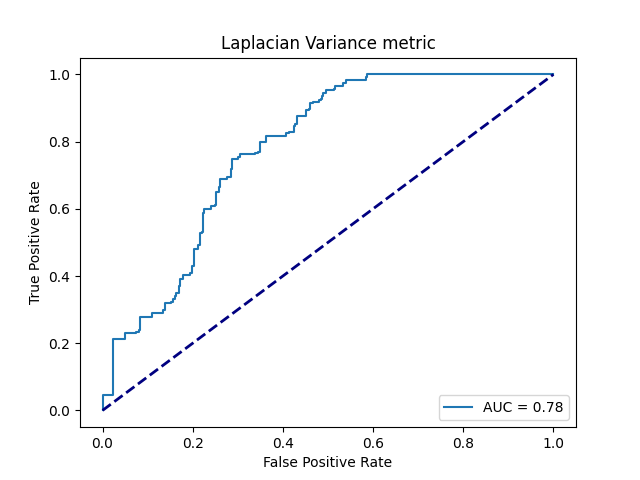
\includegraphics[width=\textwidth]{Figures/lv/output_roc_lv_png.png}
        \caption{}
        \label{fig:LV_roc}
    \end{subfigure}\hspace{1em}
    \begin{subfigure}[t]{0.48\textwidth}
        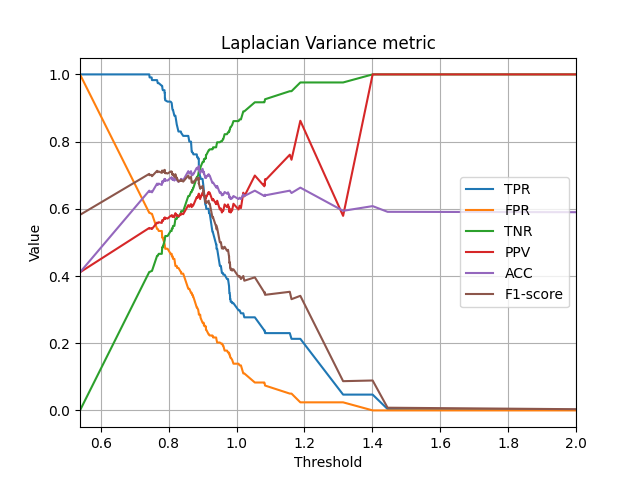
\includegraphics[width=\textwidth]{Figures/lv/threshold_test_scores_lv_png.png}
        \caption{}
        \label{fig:LV_thresh}
    \end{subfigure}\hspace{1em}
    \caption{}
    \label{fig:LV_final}
\end{figure}



\iffalse
\subsection{Combining metrics}
The three metrics, CPBD, Variance of Lapracian and Histogram Frequency-based metric, will be combined to form 4 new metrics. This is done by combining the outputs of the metrics as $m_{new}=\alpha \cdot m1 + (1-\alpha) \cdot m2$, where $m1$ and $m2$ are two different metrics.

\subsection{Merge of CPBD and Variance of Laplacian}
\textbf{Highest AUC = 90\%}
\begin{figure}[H]
    \centering
    \begin{subfigure}[t]{0.48\textwidth}
        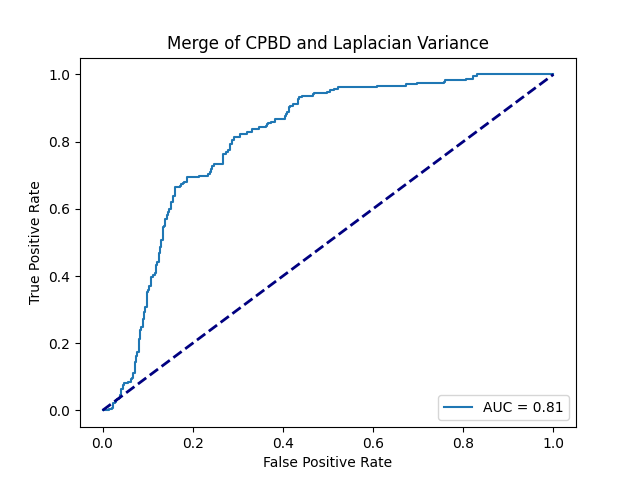
\includegraphics[width=\textwidth]{Figures/results_on_thresholds/output_roc_cpbd_lv.png}
        \caption{}
        \label{fig:CPBD_LV_roc}
    \end{subfigure}\hspace{1em}
    \begin{subfigure}[t]{0.48\textwidth}
        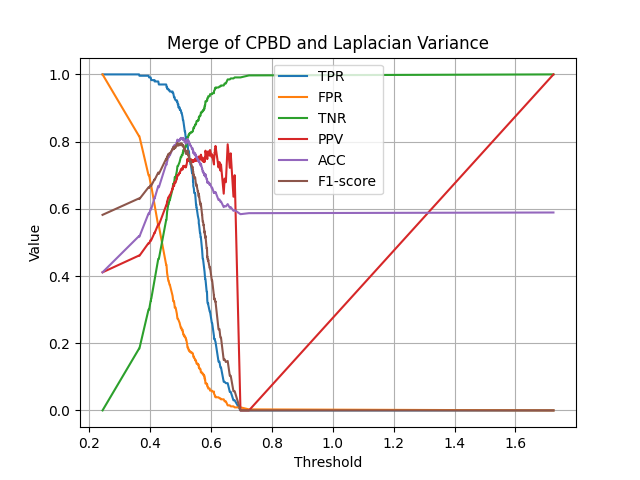
\includegraphics[width=\textwidth]{Figures/results_on_thresholds/threshold_test_scores_cpbd_lv.png}
        \caption{}
        \label{fig:CPBD_LV_thresh}
    \end{subfigure}\hspace{1em}
    \begin{subfigure}[t]{0.48\textwidth}
        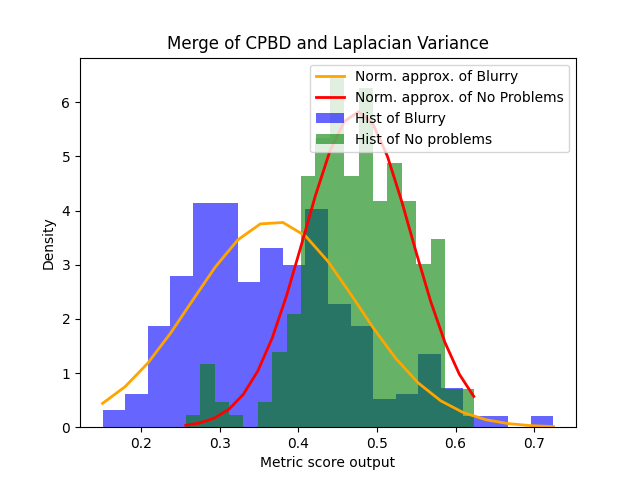
\includegraphics[width=\textwidth]{Figures/results_on_thresholds/output_dens_cpbd_lv.png}
        \caption{}
        \label{fig:CPBD_LV_dens}
    \end{subfigure}\hspace{1em}
    \caption{}
    \label{fig:CPBD_LV_final}
\end{figure}

\subsection{Merge of CPBD and Histogram frequency-based metric}
\begin{figure}[H]
    \centering
    \begin{subfigure}[t]{0.48\textwidth}
        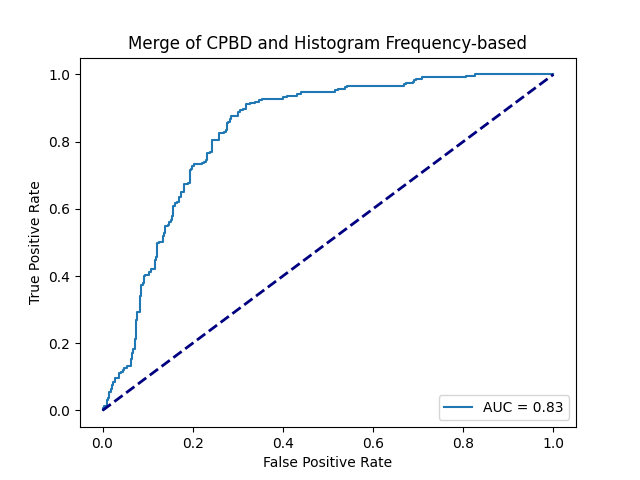
\includegraphics[width=\textwidth]{Figures/results_on_thresholds/output_roc_cpbd_hf.png}
        \caption{}
        \label{fig:CPBD_HF_roc}
    \end{subfigure}\hspace{1em}
    \begin{subfigure}[t]{0.48\textwidth}
        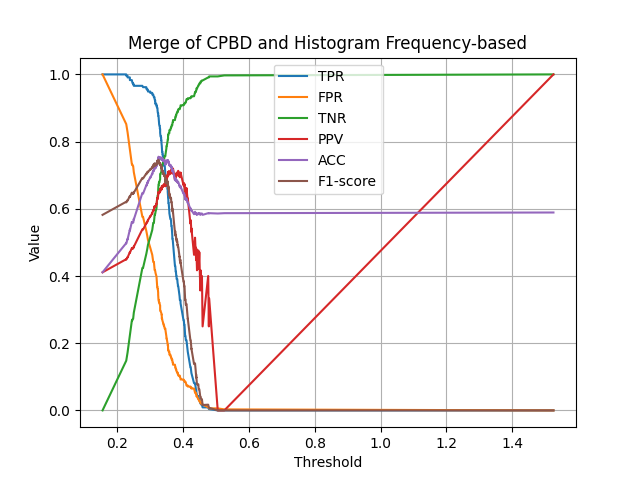
\includegraphics[width=\textwidth]{Figures/results_on_thresholds/threshold_test_scores_cpbd_hf.png}
        \caption{}
        \label{fig:CPBD_HF_thresh}
    \end{subfigure}\hspace{1em}
    \begin{subfigure}[t]{0.48\textwidth}
        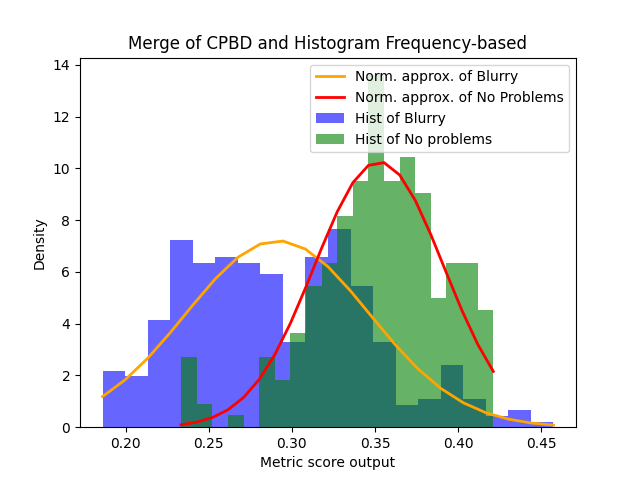
\includegraphics[width=\textwidth]{Figures/results_on_thresholds/output_dens_cpbd_hf.png}
        \caption{}
        \label{fig:CPBD_HF_dens}
    \end{subfigure}\hspace{1em}
    \caption{}
    \label{fig:CPBD_HF_final}
\end{figure}

\subsection{Merge of Histogram frequency-based metric and Variance of Laplacian}
\begin{figure}[H]
    \centering
    \begin{subfigure}[t]{0.48\textwidth}
        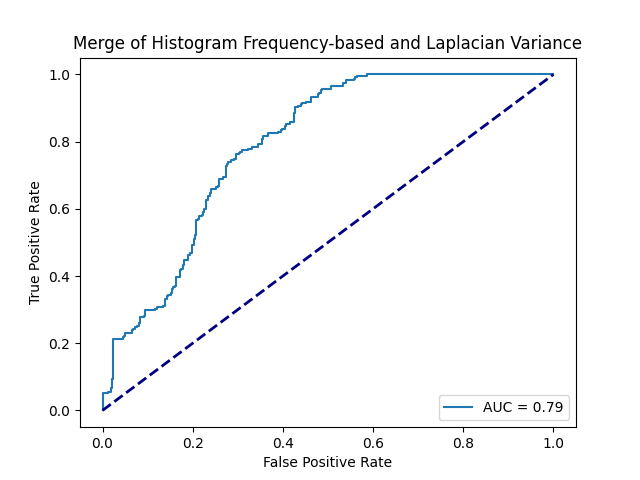
\includegraphics[width=\textwidth]{Figures/results_on_thresholds/output_roc_hf_lv.png}
        \caption{}
        \label{fig:HF_LV_roc}
    \end{subfigure}\hspace{1em}
    \begin{subfigure}[t]{0.48\textwidth}
        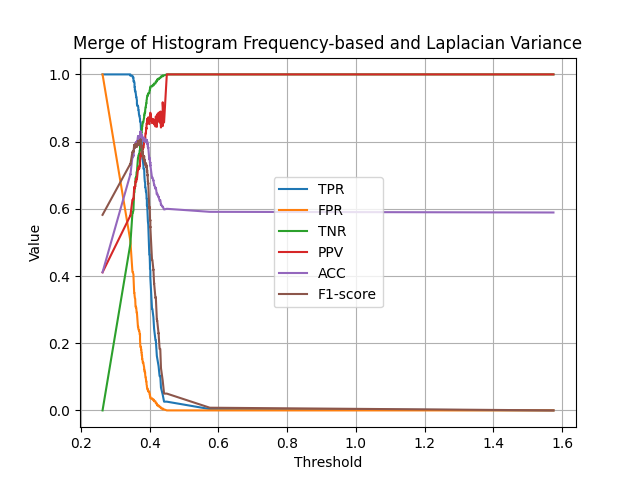
\includegraphics[width=\textwidth]{Figures/results_on_thresholds/threshold_test_scores_hf_lv.png}
        \caption{}
        \label{fig:HF_LV_thresh}
    \end{subfigure}\hspace{1em}
    \begin{subfigure}[t]{0.48\textwidth}
        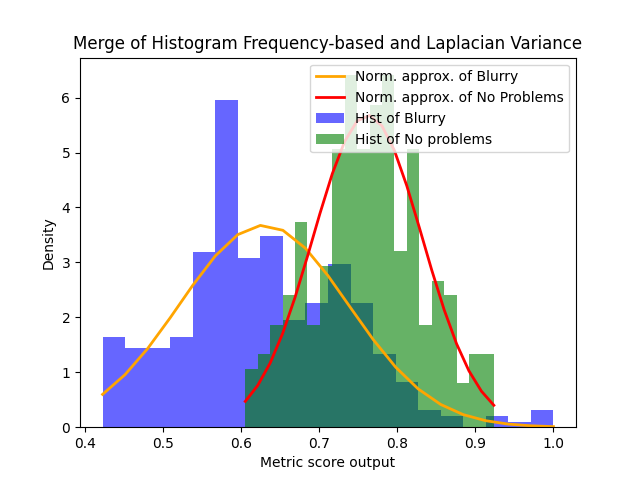
\includegraphics[width=\textwidth]{Figures/results_on_thresholds/output_dens_hf_lv.png}
        \caption{}
        \label{fig:HF_LV_dens}
    \end{subfigure}\hspace{1em}
    \caption{}
    \label{fig:HF_LV_final}
\end{figure}

\subsection{Merge of CPBD, Histogram frequency-based metric and Variance of Laplacian}
\begin{figure}[H]
    \centering
    \begin{subfigure}[t]{0.48\textwidth}
        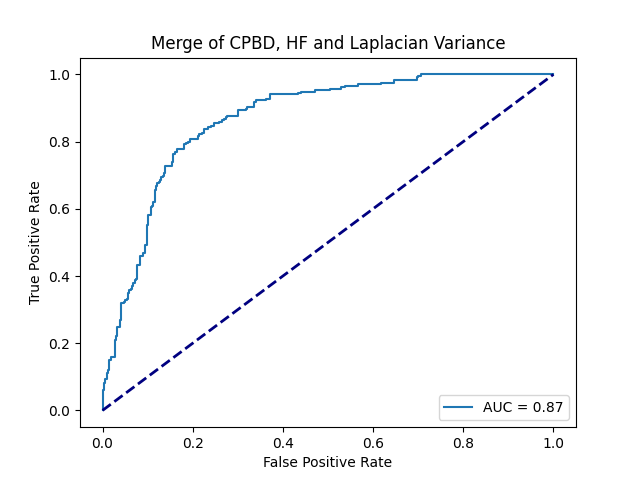
\includegraphics[width=\textwidth]{Figures/results_on_thresholds/output_roc_cpbd_hf_lv.png}
        \caption{}
        \label{fig:CPBD_HF_LV_roc}
    \end{subfigure}\hspace{1em}
    \begin{subfigure}[t]{0.48\textwidth}
        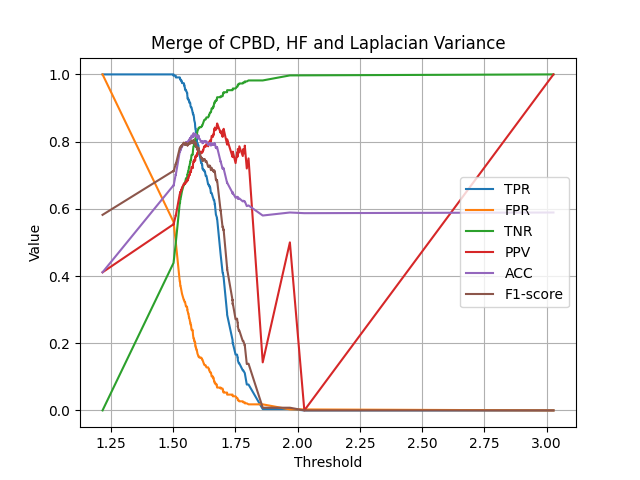
\includegraphics[width=\textwidth]{Figures/results_on_thresholds/threshold_test_scores_cpbd_hf_lv.png}
        \caption{}
        \label{fig:CPBD_HF_LV_thresh}
    \end{subfigure}\hspace{1em}
    \begin{subfigure}[t]{0.48\textwidth}
        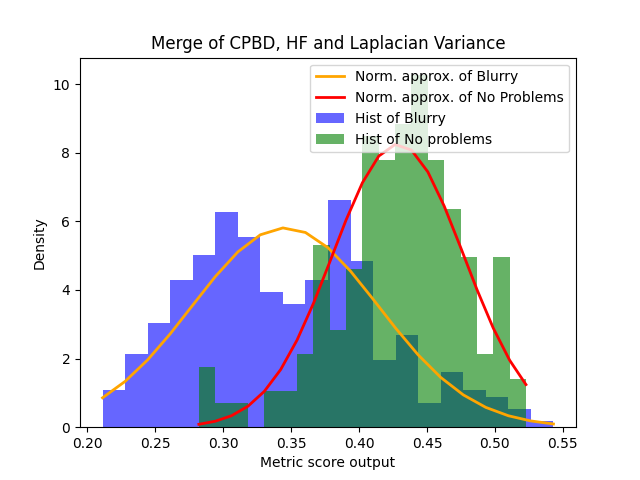
\includegraphics[width=\textwidth]{Figures/results_on_thresholds/output_dens_cpbd_hf_lv.png}
        \caption{}
        \label{fig:CPBD_HF_LV_dens}
    \end{subfigure}\hspace{1em}
    \caption{}
    \label{fig:CPBD_HF_LV_final}
\end{figure}
\fi

\subsection{"Training" the metrics}
The goal is to avoid false positives (\textbf{FP}: classified as sharp when blurry), as these can distort the results from the data later on, while still achieving some positive outputs.

\textbf{Choosing the threshold:}\\
Let the user choose an acceptable TNR (specificity), e.g. 98\%.\\
After this, find the corresponding threshold and choose the metric with the highest accuracy, as it will provide a possibility that some images will be "accepted", that is, classified as sharp. 

We could also calculate summed distance, d, of some rates... TPR (sensitivity), F1-score, precision...  to the top and bottom border (1 and 0) according to which border is desired for that particular rate. Then choose the metric with smallest d.


\begin{itemize}
    % \item minimize FPR (sharp when not) ($1-TNR$)
    \item maximize TNR (how many are blurry when blurry)
    \item maximize TPR (we would still like some possibility that images are classified "sharp")
    \item maximize PPV (part declared sharp when sharp)
    \item high f1-score for general score + do not produce FP (to not filter away too many negatives)
\end{itemize}


The following graphs displays output on the training data set excluding the Gaussian blurred images.



